%%%%%%%%%%%%%%%%%%%%%%%%%%%%%%%%%%%%%%%%%%%%%%%%%%%%%%%%%%%%%%%%%%%%%%%%%%%%%%
\documentclass[11pt,a4paper]{article}
% XXX Use this line if you want two columns
% \documentclass[10pt,a4paper,twocolumn]{article}
% This first part of the file is called the PREAMBLE. It includes
% customizations and command definitions. The preamble is everything
% between \documentclass and \begin{document}.

%% Well understand input, and nice output
\usepackage[utf8]{inputenc}
\usepackage{lmodern}
\usepackage[T1]{fontenc}

\usepackage[margin=1.00in,top=1.25in,bottom=1.25in]{geometry}  % set the margins
\usepackage{latexsym}              % symbols
\usepackage{amsmath}               % great math stuff
\usepackage{amssymb}               % great math symbols
\usepackage{amsfonts}              % for blackboard bold, etc

\usepackage{titling}
\usepackage{enumerate}
\usepackage{fixltx2e} % LaTeX patches, \textsubscript
\usepackage{cmap} % fix search and cut-and-paste in Acrobat
\usepackage{color}
\definecolor{darkgreen}{rgb}{0.0,0.55,0.0}  % Defines the color used for link


\usepackage[plainpages=false,pdfcenterwindow=true,
    pdftoolbar=false,pdfmenubar=false,
    pdftitle={TITLE},
    pdfauthor={AUTHOR},
    linkcolor=black,citecolor=black,filecolor=black,urlcolor=black]{hyperref}
     % Allows url with \href{http://truc.machin/ok?r=yes}{myref}
\usepackage{graphicx}              % to include figures
\graphicspath{{fig/}} % Directory in which figures are stored
\usepackage{caption}
\usepackage{subcaption}
\usepackage{multicol}
\usepackage{float}
\usepackage{palatino} % Use the Palatino font % XXX
\usepackage{graphics}
\usepackage{indentfirst}
\usepackage{graphicx}

% various theorems, numbered by section
\newtheorem{thm}{Theorem}[section]
\newtheorem{lem}[thm]{Lemma}
\newtheorem{proof}[thm]{Proof}

\usepackage{lastpage,fancyhdr}
\pagestyle{fancyplain}
    \renewcommand{\headrulewidth}{0.2pt}
    \renewcommand{\footrulewidth}{0.2pt}
    \lhead{\emph{Connectionist Temporal Classification}}
    %\rhead{\emph{\today}}
    \rhead{\emph{January 13, 2016}}
    \lfoot{\textsc{\'Ecole Normale Sup\'erieure de Paris}}
    \cfoot{\thepage/\pageref{LastPage}}
    \rfoot{\textsc{Alex Auvolat, Thomas Mesnard}}

%% Horizontal Lines
\providecommand*{\hr}[1][class-arg]{%
    \hspace*{\fill}\hrulefill\hspace*{\fill}
    \vskip 0.65\baselineskip
}


%%%%%%%%%%%%%%%%%%%%%%%%%%%%%%%%%%%%%%%%%%%%%%%%%%%%%%%%%%%%%%%%%%%%%%%%%%%%%%
\begin{document}
\DeclareGraphicsExtensions{.pdf,.png,.jpg}

\pretitle{
    \begin{center}
    \vspace{-5em}
    \includegraphics[width=3cm]{ens2.jpg}\hfill
    \includegraphics[width=3cm]{ENSCachan.png}\hfill
    \includegraphics[width=3cm]{mila.png}\\\vspace{3em}
}
\posttitle{\end{center}}
% 
%------------------------------------------------------------------------------
\title{\huge Connectionist Temporal Classification: \\Labelling Unsegmented Sequences with \\Recurrent Neural Networks \\ \Large{Research Project Report -- Probabilistic Graphical Models course} }
% \date{\today}
\date{}

\maketitle
% ------------------------------------------------------------------------------
% \vspace*{-1.5cm}
\begin{center}
% Authors
    \begin{multicols}{2}
        \setcounter{footnote}{-1}  %% XXX
        \textsc{Alex Auvolat} \\
            Department of Computer Science\\
            \'Ecole Normale Sup\'erieure de Paris \\
            \texttt{alex.auvolat@ens.fr}\\
        \textsc{Thomas Mesnard}
            \footnote{If needed, see online at \url{https://github.com/thomasmesnard/CTC-LSTM} for the implementation, open-sourced under the Apache license.}\\
            Department of Computer Science\\
            \'Ecole Normale Sup\'erieure de Paris \\
            \texttt{thomas.mesnard@ens.fr}\\
        % \and  % \and or \And or \AND
    \end{multicols}
    %\vspace*{-0.3cm}
    %    \'Ecole Normale Sup\'erieure de Paris \\
    %    \texttt{\{alex.auvolat,thomas.mesnard\}@ens.fr}
\end{center}

\vspace{1em}

% ------------------------------------------------------------------------------
\hr{}  % Horizontal line, like <hr> in HTML
%\hfill{}

\vspace{1em}

% ------------------------------------------------------------------------------
% A small abstract of what is done in the paper
\begin{abstract}
    Many real-world sequence learning tasks require the prediction of sequences of
    labels from noisy, unsegmented input data. Recurrent neural networks (RNNs) are powerful sequence learners that would seem well suited to such tasks. However, because they require pre-segmented training data, and post-processing to transform their outputs into label sequences, they cannot be applied directly. Connectionist Temporal Classification is a method for training RNNs to label unsegmented sequences directly, thereby solving both problems.
\end{abstract}

\vspace{1em}

% ------------------------------------------------------------------------------
\hr{}  % Horizontal line, like <hr> in HTML
% XXX remove if it is ugly or take too much space

%\hfill{}

\vspace{1em}

% ------------------------------------------------------------------------------
% About the report
\begin{center}
        \textbf{Project Advisor:} Guillaume Obozinski \\
        \textbf{Course:}
        \emph{``Probabilistic Graphical Models''}, by F. Bach, S. Lacoste-Julien, G. Obozinski \\
        \textbf{For} the \href{http://www.math.ens-cachan.fr/version-anglaise/academics/mva-master-degree-227777.kjsp}{Math\'ematiques, Vision, Apprentissage (MVA)} Master 2
        at \href{http://www.ens-cachan.fr/}{ENS de Cachan}.
\end{center}

%\footnote{If needed, see online at \href{https://github.com/thomasmesnard/CTC-LSTM}{https://github.com/thomasmesnard/CTC-LSTM}for an e-version of this report, as well as additional resources, open-sourced under the \href{http://opensource.org/licenses/MIT}{MIT License}}

%%%%%%%%%%%%%%%%%%%%%%%%%%%%%%%%%%%%%%%%%%%%%%%%%%%%%%%%%%%%%%%%%%%%%%%%%%%%%%
\newpage

\section{Model}

Connectionist Temporal Classification (CTC) introduces a new cost function for training recurrent neural networks to label unsegmented sequences directly.
To use this cost function, we introduce an additional blank symbol in the possible labels that the recurrent neural networks can output. We remind that the output layer of the recurrent neural networks correspond to probabilities over all possible labels.

This additional blank symbol give freedom to the RNN to give the label for a section of input at any moment, and especially when it is sure of its answer, simply by outputting the blank label the rest of the time.

The blank label also allows the network to give a strong probability to the correct label at a very localized point in time, whereas in a classical setup we observe distributed probabilities over all labels at each time step. An example of both behaviors can be observed on speech data in Figure \ref{Example}.

\begin{figure}[h]
    \centering
    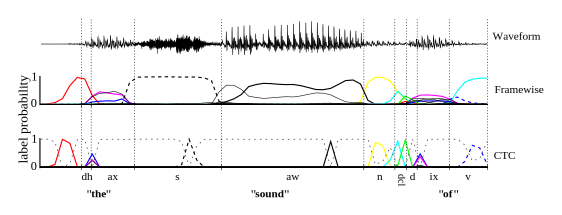
\includegraphics[width=1\linewidth]{azerty3.png}
    \caption{\small Output of classic framewise phoneme classification and RNN trained with CTC}
    \label{Example}
\end{figure}

As the output sequence is shorter than the input sequence, there are many possible alignments with the correct label sequence. We want the recurrent neural network to learn one of these correct alignments on its own. Using dynamic programing to sum over all the possible alignments, CTC provides gradients for the backpropagation phase to train the RNN to learn a good alignment.

In the basic setup shown in Figure~\ref{Setup}, we use stacked bidirectional recurrent neural networks. The CTC brick takes as inputs the output of the last bidirectional recurrent neural network as well as the target label sequence, and calculates the cost of the label. When differentiated, the CTC brick gives back gradients to train the RNN and learn a good alignment.


% \begin{figure}[h]
%     \centering
%     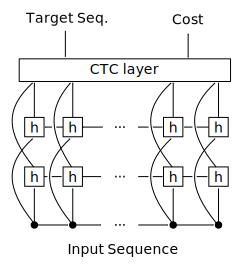
\includegraphics[width=0.3\linewidth]{azerty4.png}
%     \caption{Simple bidirectional RNN model with CTC cost layer}
%     \label{Setup}
% \end{figure}

We use the following notation:

\begin{itemize}
    \item $y_k^t$: output at time $t$ for symbol $k$
    \item $l$: the label sequence for which we want to calculate a cost
	\item $l'$: the same label sequence but with blanks added between each letters
\end{itemize}

\begin{figure}[H]
    \hfill{}
    \begin{minipage}{.4\textwidth}
        \centering
        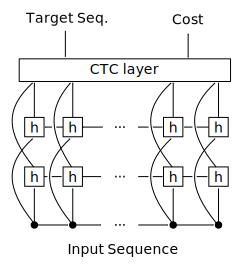
\includegraphics[width=0.8\linewidth]{azerty4.png}
        \caption{Simple bidirectional RNN model with CTC cost layer}
        \label{Setup}
    \end{minipage}
    \hfill{}
    \begin{minipage}{.5\textwidth}
        \centering
		\vspace{1em}
        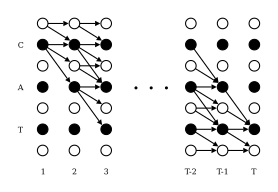
\includegraphics[width=1.0\linewidth]{azerty1.png}
        \caption{Computation graph for $\alpha_t(s)$ (corresponds to an unrolling of the automaton that recognizes $\mathcal{B}^{-1}(l)$)}
        \label{auto}
    \end{minipage}
    \hfill{}
\end{figure}

\subsection{First Definition}

CTC is a dynamic programming algorithm that calculates the following variable:

\begin{equation}
    \alpha_t(s) = \sum_{\substack{\pi \in N^T:\\\mathcal{B}(\pi_{1:t}) = l'_{1:s}}}              \prod_{t'=1}^t y_{\pi_{t'}}^{t'} 
    \label{first}   
\end{equation}

Where: 
\begin{itemize}
    \item $\mathcal{B}$ is the transform that removes all blanks and duplicates
    \item $\pi \in N^T: \mathcal{B}(\pi_{1:t}) = l'_{1:s}$ corresponds to all possible paths among all possible labels from time step $1$ to $t$ which give the $s$ first correct labels after we apply the $\mathcal{B}$ transform.
    \item $y^{t'}$ corresponds to the output of the RNN at time $t'$ 
\end{itemize}

We can see that $\alpha_t(s)$ corresponds to the sum, over all possible paths between time step $1$ and $t$ that will give the $s$ first correct labels after removing all banks and duplicates, of the product of the probabilities output by the RNN on these paths.

The formulation described in Equation~\ref{first} is equivalent to the unrolled automaton presented in Figure~\ref{auto}. 
To allow for blanks in the output paths, we consider a modified label sequence $l'$, with blanks added to the beginning and the end and inserted between every pair of labels. The length of $l'$ is therefore $2|l|+1$. This allows transition  between blank and non-blank labels, and also those between any pair of distinct non-blank labels.

% \begin{figure}[h]
%     \centering
%     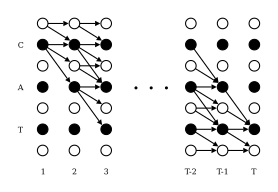
\includegraphics[width=0.6\linewidth]{azerty1.png}
%     \caption{Computation graph for $\alpha_t(s)$ (corresponds to an unrolled automaton)}
%     \label{auto}
% \end{figure}


\subsection{Recursive Definition}

The definition of $\alpha_t(s)$ given above enables us to understand what this function calculates, but unfortunately it is not practical to compute. We will now see a recursive definition of the $\alpha_t(s)$ which provides a dynamic programming algorithm for our problem. This calculation is illustrated in Figure~\ref{auto}.

We first have to initiate $\alpha_1$ with at first a blank label, then the first correct label and finally just zeros. Indeed, it is impossible that more than one correct label derive from only one output of the RNN:

\[
\begin{tabular}{rcl}
    $\alpha_1(1)$ &=& $y_b^1$\\
    $\alpha_1(2)$ &=& $y_{l_1}^1$\\
    $\alpha_1(s)$ &=& $0, \forall s > 2$
\end{tabular}
\]

We then define the recurrence relations:
\[
\alpha_t(s) = 
\begin{cases}
    \bar{\alpha}_t(s) y_{l'_s}^t & \mbox{ if } l'_s = b\mbox{ or }l'_{s-2}=l'_s \\
    (\bar{\alpha}_t(s)+\alpha_{t-1}(s-2)) y_{l'_s}^t &\mbox{ otherwise}\\
\end{cases}
\]

With:

\[
\bar{\alpha}_t(s) = \alpha_{t-1}(s) + \alpha_{t-1}(s-1)
\]

Finally, we have:
\[
    p(l|x) = \alpha_T(|l'|) + \alpha_T(|l'|-1)
\]

Which give us, given an input, the probability of having a particular sequence.


\subsection{Analysis of the Gradient Provided by CTC}

\begin{figure}[h]
    \centering
    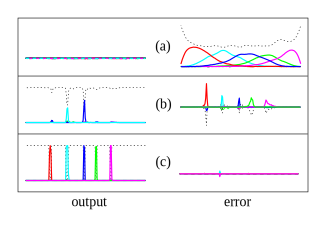
\includegraphics[width=0.6\linewidth]{azerty2.png}
    \caption{Evolution of the CTC error signal}
    \label{error}
\end{figure}

In Figure \ref{error}, the left column shows the output activations for the same sequence at various stages of training. The dashed line corresponds to the blank unit. The right column shows the corresponding error signals, i.e.~the gradient which is sent back to the RNN.

On the early stage of the training (a), the network does not make predictions because it has small random weights, the error is only determined by the target sequence and is localized only very vaguely.

During the training (b), the network begins to make predictions and the error localizes around them.

At the end of the training (c), the network strongly predicts the correct labels at very specific times, and the rest of the time outputs the blank label. The error signal becomes null since there is no error.


\section{Experiments}

We made an implementation of the model using \href{https://github.com/Theano/Theano}{Theano} and \href{https://github.com/mila-udem/blocks/}{Blocks} which is a Theano framework for building and training neural networks. The code is available at the following address: \url{https://github.com/thomasmesnard/CTC-LSTM}.

As Theano provides an automated symbolic differentiation tool, we implemented the forward recursion for $\alpha_t(s)$ and let Theano derive the backward calculation. To avoid numerical underflow, two methods can be applied, which we both implemented:

\begin{itemize}
    \item Normalize at each time step $t$ the $\alpha_t$:
    \hspace{1em}
    $ C_t = \sum_s \alpha_t(s)$
    \hspace{1em}
    $\hat{\alpha}_t(s) = \frac{\alpha_t(s)}{C_t}$
    \item Do our calculations in the logarithmic domain

\end{itemize}

\subsection{Toy Dataset}

We first tried our implementation on a simple task. Our dataset is composed of the following sequences, where each digit is randomly repeated a random number of times.

\begin{center}
\begin{tabular}{c}
    $1^*2^*3^*4^*5^* \to 1$  \\
    $1^*2^*3^*2^*1^* \to 2$  \\
    $5^*4^*3^*2^*1^* \to 3$  \\
    $5^*4^*3^*4^*5^* \to 4$  \\
\end{tabular}
\end{center}

The network has to learn the previous association. The two first sequences have an overlap on the three first digits. The network has to wait until the fourth digit to know if it is either a 1 or a 2. We can see here the importance of the blank label. Indeed, the network will have to outputs the blank label until the fourth label is presented to be able to give the correct label. The same reasoning can be applied for the two last sequences.

We have two versions of the toy dataset: on the first version each piece of the sequence is perfectly identifiable as each character appears at least once (the input sequence is therefore at least 5 times as long as the target sequence). On the second version some characters may be omitted in the input, adding stochasticity to the task. CTC provides very good results on the two tasks (shown in Table~\ref{tbl_result} and Table~\ref{tbl_result2}).

\begin{table}[H]
    \centering
    \vspace{2ex}
	\begin{minipage}{0.45\textwidth}
    \begin{tabular}{l l l}
        %\toprule
		\hline
        \textbf{Results} & \textbf{train} & \textbf{valid}\\ 
		\hline
        %\midrule
        Output sequence length & 5 -- 50 & 5 -- 50 \\
        Error rate & 0 & 0 \\
        Mean edit distance & 0 & 0 \\ 
        Errors per character & 0 & 0 \\
		\hline
        %\bottomrule
    \end{tabular}
    \caption{Performances of CTC on our toy dataset, with perfect input sequences}
	\label{tbl_result}
	\end{minipage}
	\hfill{}
	\begin{minipage}{0.45\textwidth}
    \begin{tabular}{l l l}
        %\toprule
		\hline
        \textbf{Results} & \textbf{train} & \textbf{valid}\\ 
		\hline
        %\midrule
        Output sequence length & 5 -- 20 & 5 -- 20 \\
        Error rate & 0.62 & 0.63 \\
        Mean edit distance & 1.0 & 1.1 \\ 
        Errors per character & 0.08 & 0.09 \\
		\hline
        %\bottomrule
    \end{tabular}
    \caption{Performances of CTC on our toy dataset, with imperfect input sequences}
	\label{tbl_result2}
	\end{minipage}
\end{table}

We observe that the model performs flawlessly on the first task. On the other task, the error rate is not as low as expected but we remind that it corresponds to the rate on which the network is able to find the complete target sequence. A more meaningful measure is the error rate per character which is only $9\%$ on the validation set. We deduce from these two results that the model is able to perfectly learn the rule that maps the input sequences to the targets, but even though, it cannot achieve perfect results on the second task as information is sometimes missing in the input. Both implementations converge in less than 1000 time steps. 

%\begin{figure}[h]
%    \centering
%    \includegraphics[width=0.6\linewidth]{ctc_cost_best.png}
%    \caption{Training and validation cost of the CTC model (negative log likelihood)}
%\end{figure}

\subsection{TIMIT}

\begin{figure}[H]
    \hfill{}
    \begin{minipage}{.5\textwidth}
        \centering
        \includegraphics[width=0.95\linewidth]{pouet_timit_cost.png}
        \caption{\footnotesize Training cost of the CTC model on TIMIT}
        \label{timit_cost}
    \end{minipage}
    \hfill{}
    \begin{minipage}{.45\textwidth}
        \centering
		\vspace{1em}
        \includegraphics[width=0.95\linewidth]{pouet_timit_ER.png}
        \caption{\footnotesize Error rate of the CTC model on TIMIT}
        \label{timit_er}
    \end{minipage}
    \hfill{}
\end{figure}


\begin{table}[H]
	\centering
	\small
    \begin{tabular}{l l l l l l}
		\hline
		\textbf{Convolution layers} & \textbf{Filters} & \textbf{Filter size} & \textbf{Stride} & \textbf{Skip} & \textbf{Normalize} \\
		\hline
		Layer 1 & 20 & 200 & 10 & Yes & Yes \\
		Layer 2 & 20 & 200 & 10 & Yes & Yes \\
		Layer 3 & 20 & 30 & 2 & Yes & Yes \\
		Layer 4 & 100 & 20 & 2 & No & Yes \\
		\hline
		\textbf{Recurrent layers} & \textbf{Size} & \textbf{Type} & \textbf{Bidirectional} & \textbf{Skip} & \textbf{Normalize} \\
		\hline
		Layer 1 & 50 & LSTM & Yes & Yes & No \\
		Layer 2 & 50 & LSTM & Yes & Yes & No \\
		\hline
        %\bottomrule
    \end{tabular}
	\caption{Structure of the Deep Neural Network for the TIMIT dataset}
	\label{params_timit}
\end{table}

We then tried on the classical TIMIT dataset. It is a raw speech signal dataset of 4120 sentences labelled by phonemes or by words. The average audio length is 50\,000 samples and the average sentence length is 38 phonemes.

To avoid hand-crafted feature extraction on the speech signal, we use convolution layers before the bidirectional LSTM layers. We then use bidirectional LSTM layers, and of course the CTC cost function. We use noise and normalization on intermediate layers for regularization. The structure of our model is described in Table~\ref{params_timit}.

We were able to attain a $50\%$ phoneme error rate on the validation set after about 150 epochs of training (see Figure~\ref{timit_er}). This result is not as good as the $30\%$ achieved by the original paper~\cite{graves2006connectionist}, however it is an extremely good result for the model as we do not use hand-crafted preprocessing on the data. This shows that the convolution layers are able to learn the filters necessary for audio processing on speech by themselves.

\section{Conclusion}

CTC is a powerful cost function for training RNNs on unsegmented data, now largely used in major commercial applications. We were able to get very good results using CTC on a toy dataset. We proposed a way of processing speech data with convolutional neural networks and were able to train a convnet-LSTM-CTC model with satisfactory results on TIMIT.
% ------------------------------------------------------------------------------
% ------------------------------------------------------------------------------

%\vspace{4em}
%\hr{}  % Horizontal line, like <hr> in HTML
%\vspace{2em}

% XXX remove if it is ugly or take too much space


%% Bibliography
\nocite{*}  % XXX remove to hide references not cited!

% To compile: pdflatex, pdflatex, bibtex, pdflatex, pdflatex
\bibliographystyle{unsrt}

\small
\bibliography{Report}


% ------------------------------------------------------------------------------
%\hr{}  % Horizontal line, like <hr> in HTML
% XXX remove if it is ugly or take too much space


%\vfill
%\subsubsection*{License}
%\begin{center}
%    \begin{small}
%        This paper (and the additional resources -- including code, images, etc),
%        are publicly published under the terms of the \href{http://opensource.org/licenses/MIT}{MIT License}.
%        Copyright 2015-2016 \copyright ~Alex~Auvolat and ~Thomas~Mesnard.
%    \end{small}
%\end{center}


\end{document}
